\newpage
\section{Background}
Knowit uses an agile work form. The broader perspective for Knowit of creating a web application, not taking the iterative part of the process into account, is done in three main steps, shown in figure \ref{fig:ddp}. 
% \begin{enumerate}
%   \item Design
%   \item Develop 
%   \item Publish
% \end{enumerate}

\begin{figure}[H]
  \centering
  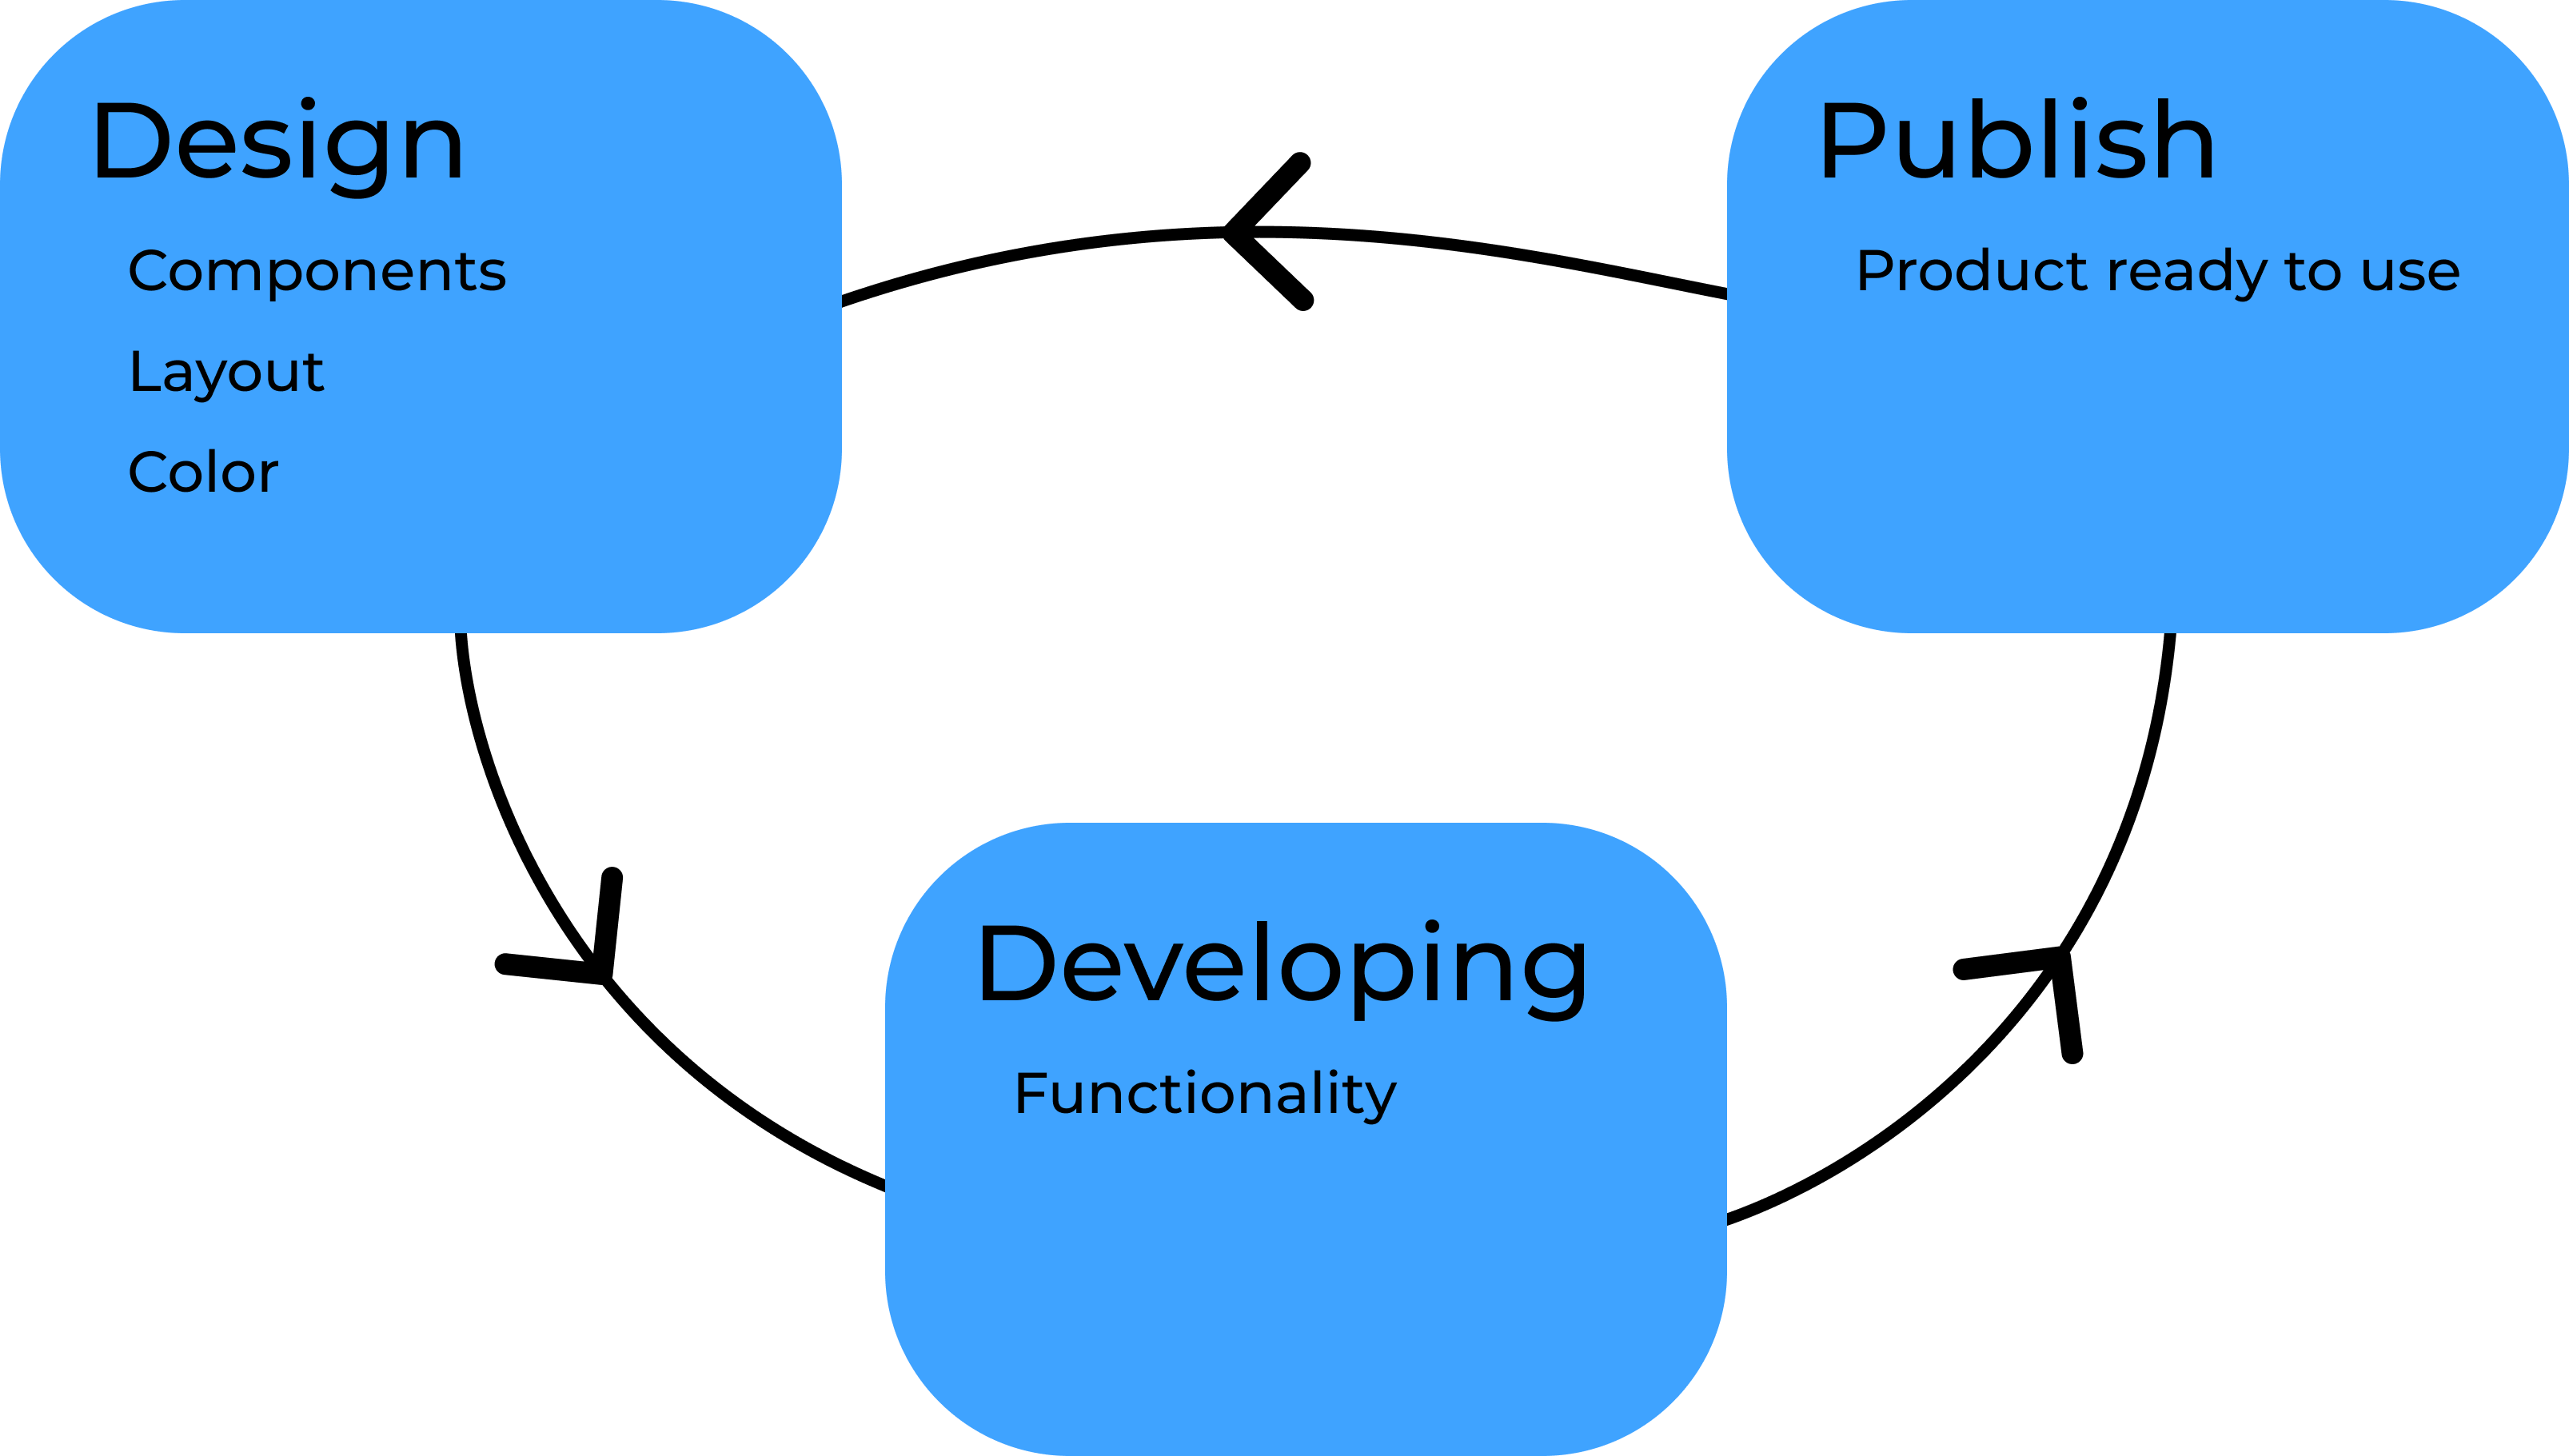
\includegraphics[width=0.8\linewidth]{images/ddp.png}
  \caption{Simplified view over the process of making a web-application}%
  \label{fig:ddp}
\end{figure}


\textbf{Design:} The designer does most design work at the beginning of the project. The designer and customer collaborate to create an interface until they are satisfied. This collaboration can be done in person, where the designer draws on paper and the customer has insight. The collaboration is often done via online software, such as Figma\cite{FigmaCollaborativeInterface}, where the designer can share the design and the customer can write comments. During this first part of the process, some developers are also present to give insight into what is possible to create for the desired system. This process results in a complete design of the application. 

\textbf{Develop:} Generally, the development that starts at the beginning of the project is primarily functional (back-end development), meaning there is no graphical interface yet. Then, when the customer has approved the design, the development starts on the visual parts of the system (front-end development). This process connects the functionality created by the back-end and design to make a functional application.

\textbf{Publish:} When the web application is at the point that the customer, designer, and developers are satisfied, the application can be published. When the application is published, the customer's users have access to it. For most projects, the customer stays in touch with the designer and developers to manage the application. Management consists of fixing bugs, updating functionality, adding features, and updating features.

\subsection{Prototype data flow}%
\label{sub:Prototype data flow}
The resulting tool from this project will follow the before mentioned steps except publish. The generated \glspl{component} are not a complete web application and should not, therefore, be published to web. However, the generated \glspl{component} need to be distributed between designer and developer. Therefore \textit{publish}, for this project is replaced by \textit{distribute}. 

All these steps are often, if not always, done iteratively. However, there must be some design to start a meaningful and valuable development effort. If there is nothing that has been developed, there is nothing to publish. Therefore these three, design, develop, distribute must be done in order. 

The resulting tool from this project adjoins all three steps. 
\begin{enumerate}
  \item Design - Using the UI program Figma
  \item Develop - With Figmas API and generator prototype
  \item Distribute - By copying files or using a package manager 
\end{enumerate}
A data flowchart for the system is shown in figure \ref{fig:flow}.

\begin{figure}[H]
  \centering
  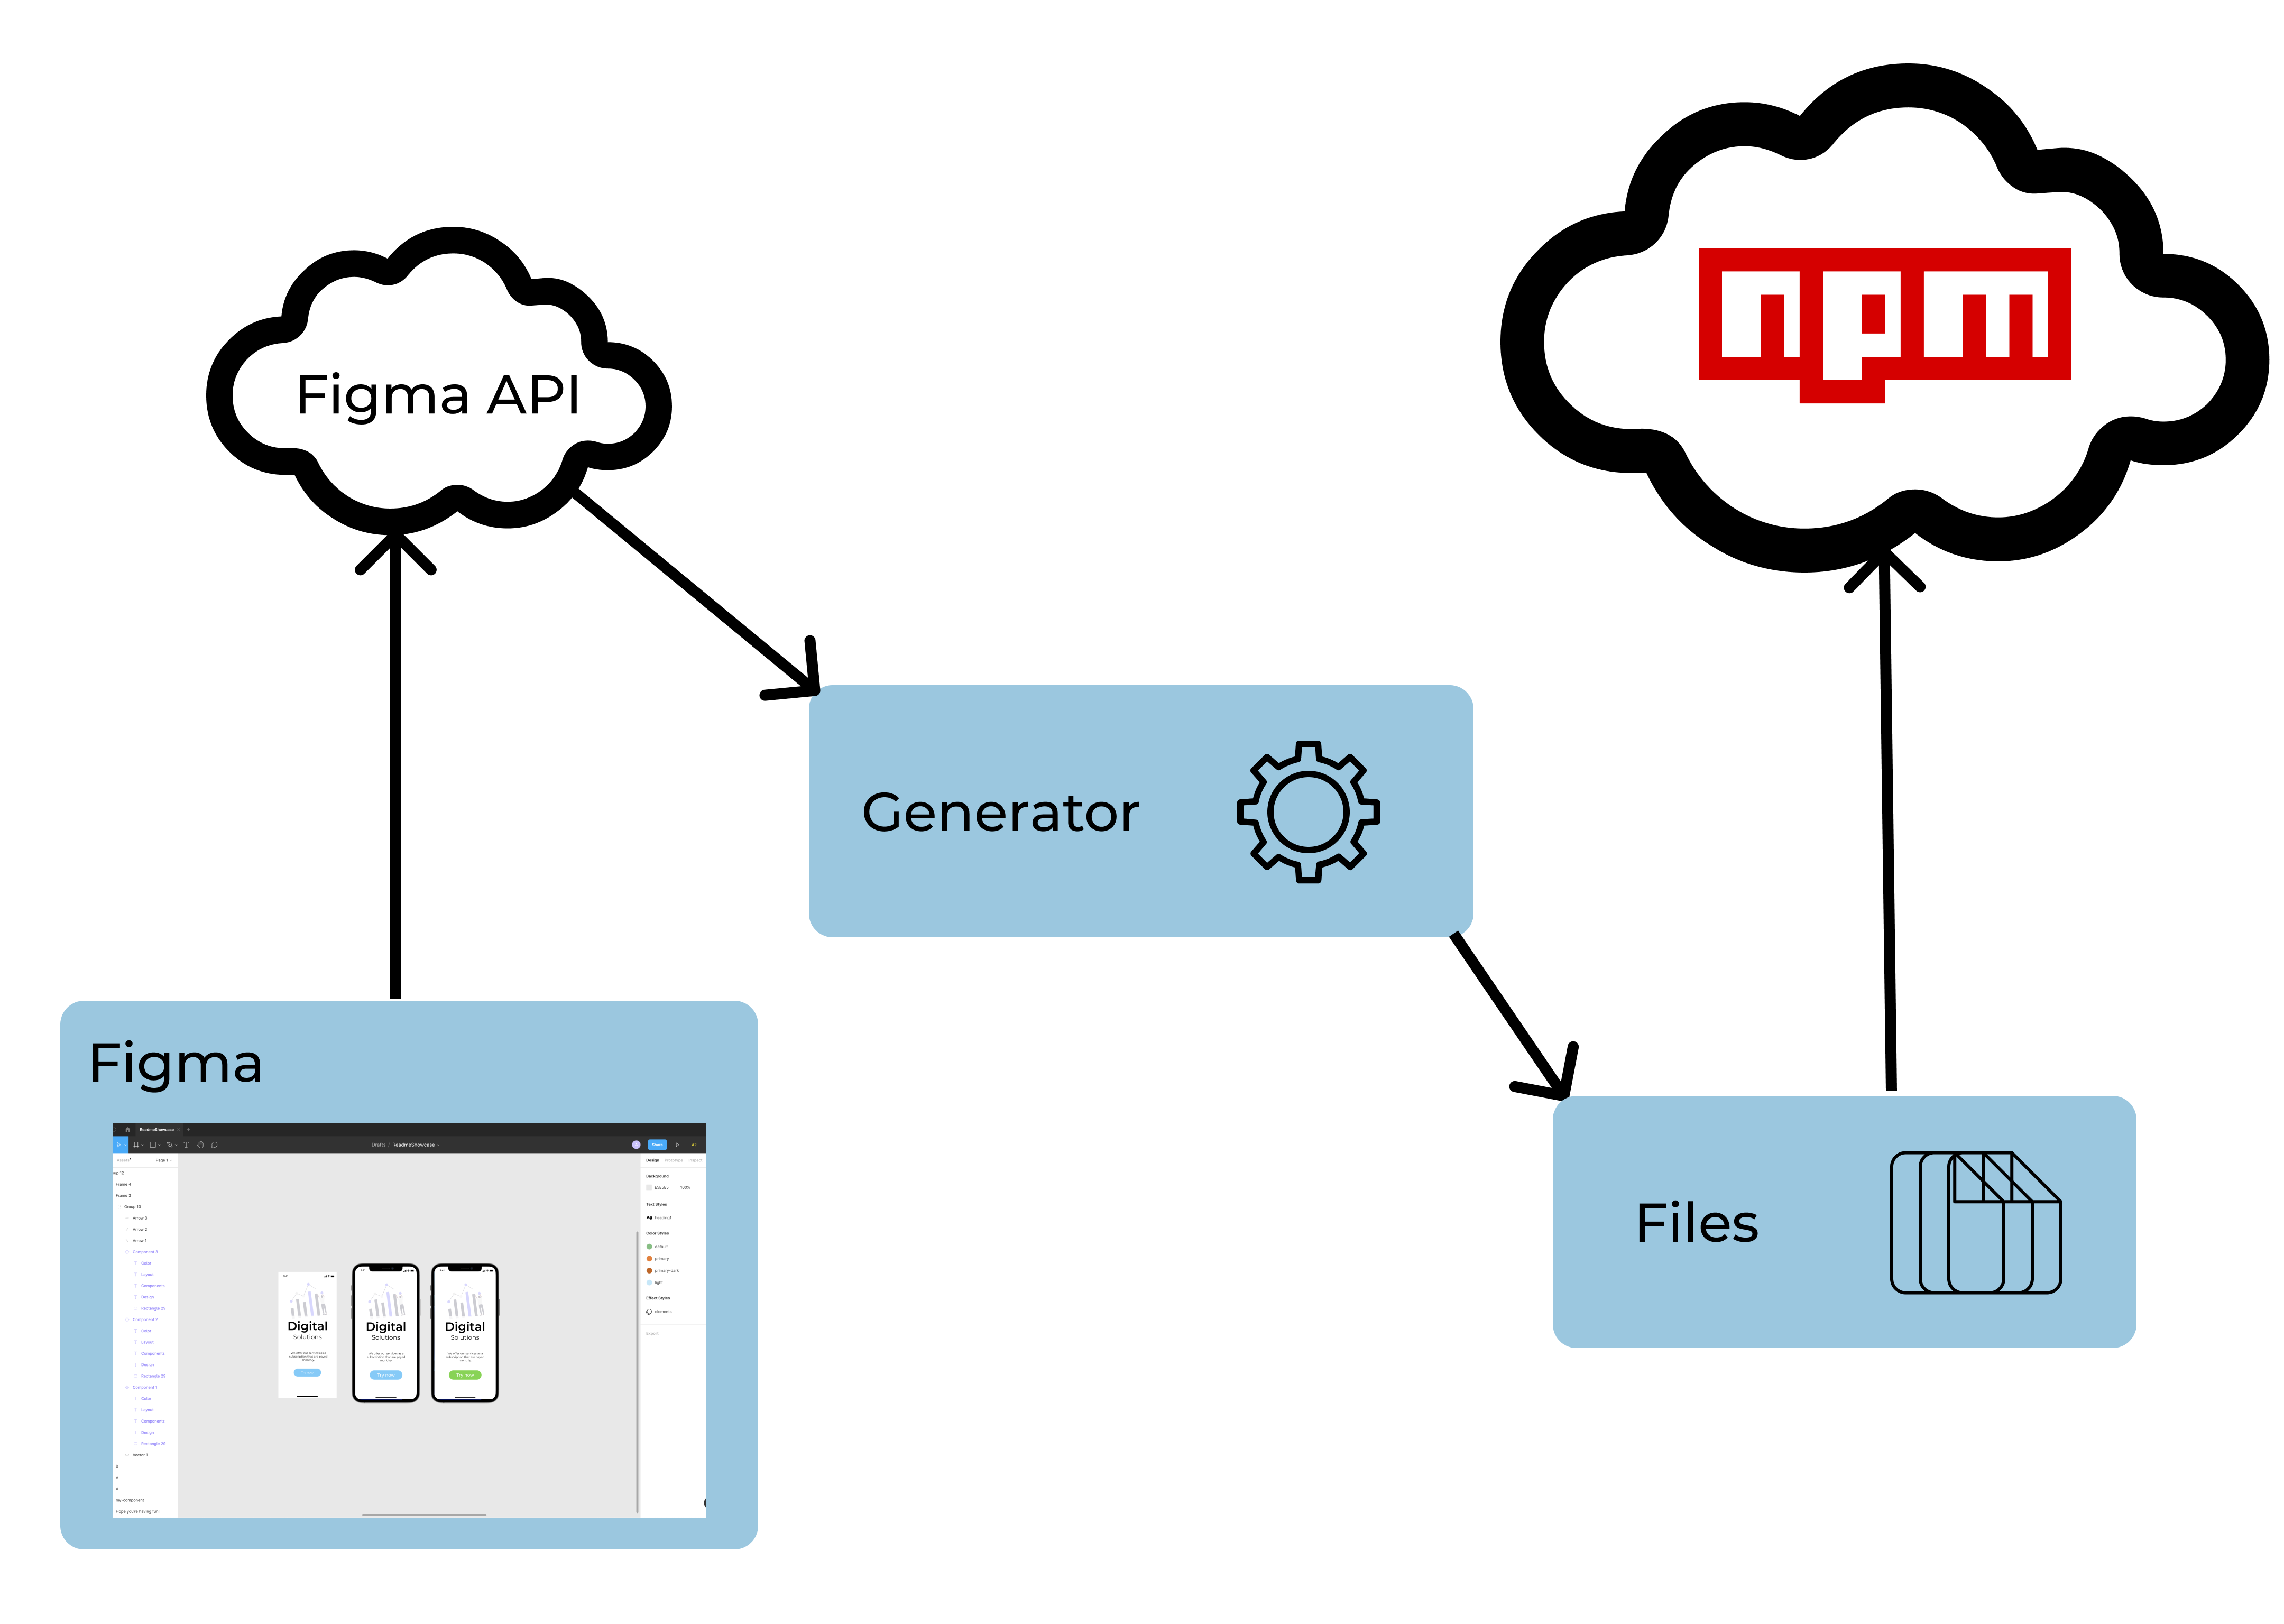
\includegraphics[width=0.8\linewidth]{images/flow2.png}
  \caption{Flowchart for data flow in the system.}%
  \label{fig:flow}
\end{figure}


\subsection{Competitors}%
\label{sub:Competitors}
The idea of making a design software generate functional code is not new. To get inspired and understand how these software work, we will look at two competitors in this field. 

\subsubsection{Webflow}
Webflow was founded in 2013 and is a product of the famous Y Combinator program\cite{Combinator}. Webflow allows the user to design, create and publish a website all from their web application. Webflow is a visual editing tool. The user does not need to know how to program since Webflow generates HTML, CSS, and JavaScript from the design. Most \acrshort{ui} applications let the user move elements freely around the canvas. Webflow is a more static build tool where the elements in the design \textit{snap} in place. Most of the design is made using the control panel, which can be observed in the right in figure \ref{fig:webflow}, and not on the canvas itself \cite{ResponsiveWebDesign}. 

\begin{figure}[H]
  \centering
  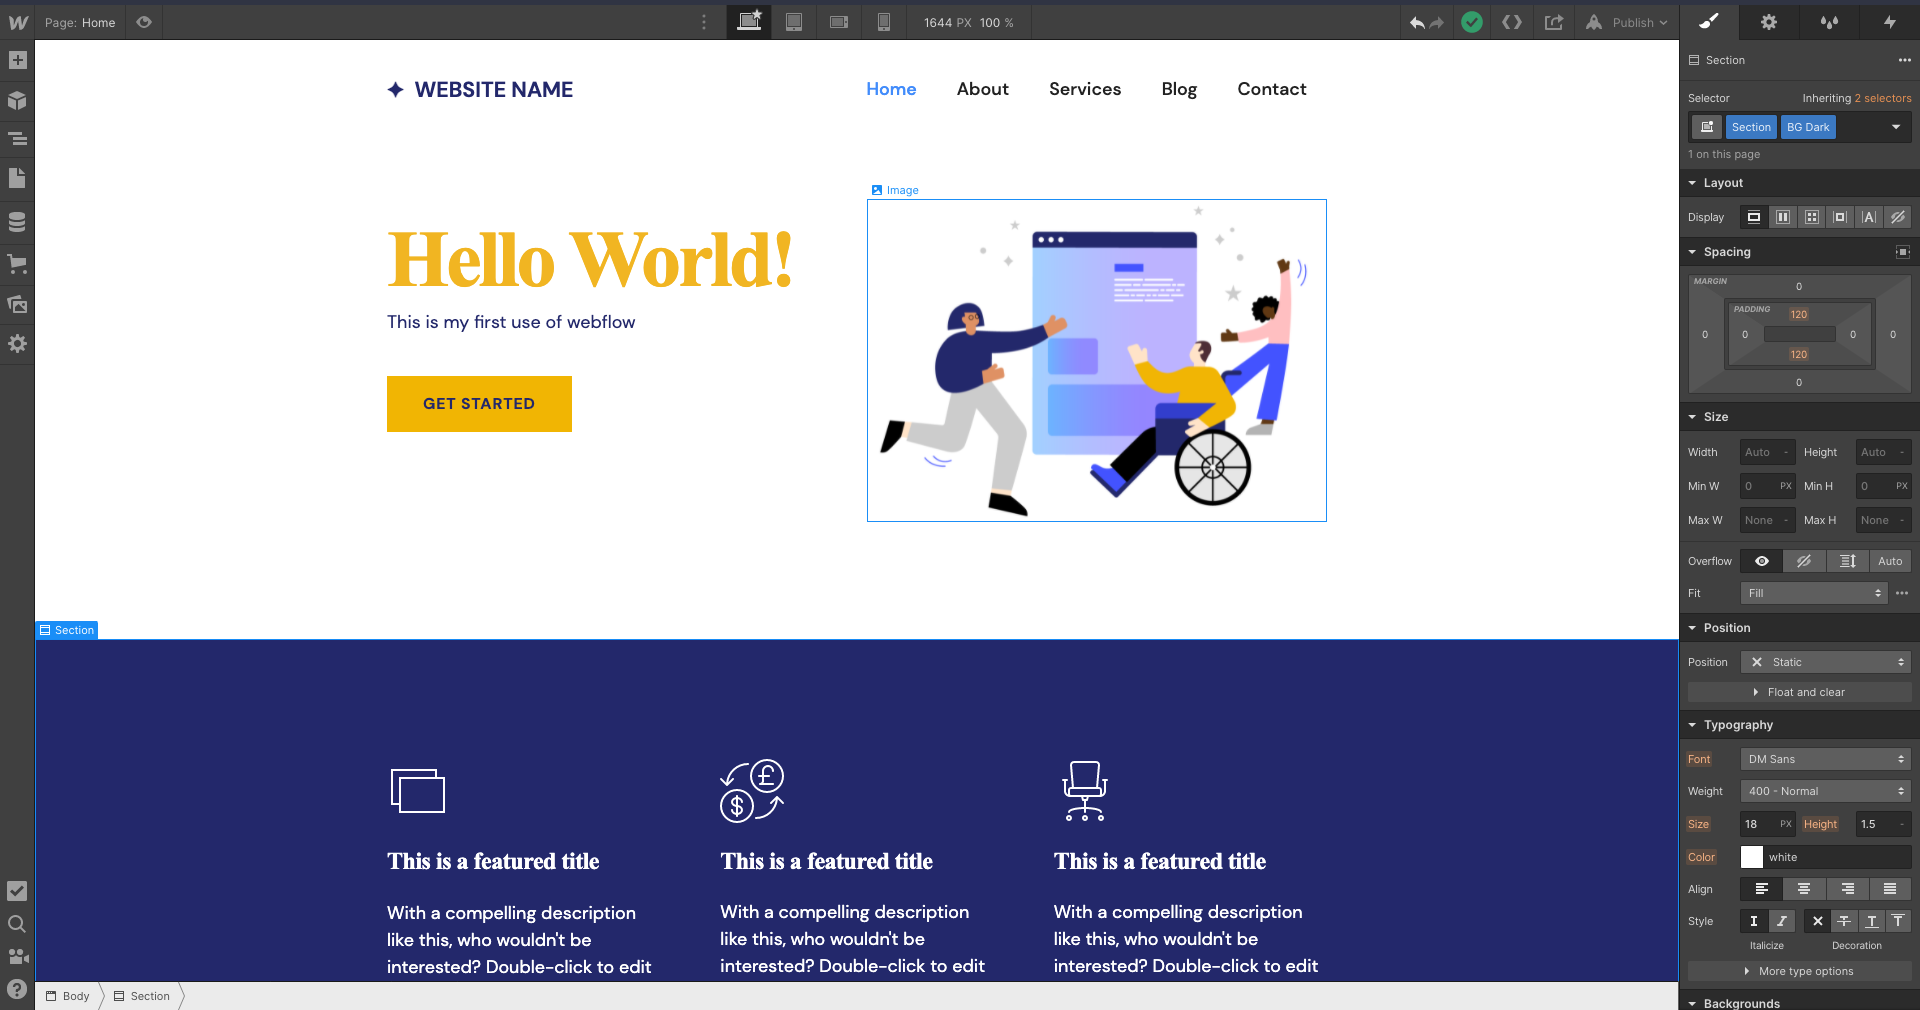
\includegraphics[width=0.8\linewidth]{images/webflow.png}
  \caption{Screenshot of Webflows UI}%
  \label{fig:webflow}
\end{figure}

\subsubsection{Visly}%
\label{ssub:Visly}
Visly was founded in 2018 and creates React \glspl{component} \cite{facebookincReactJavaScriptLibrary} from the the created design. React is a component-based JavaScript library made by Facebook. Visly essentially makes it possible to create these \glspl{component} visually. 

\begin{figure}[H]
  \centering
  \includegraphics[width=0.8\linewidth]{images/visly.png}
  \caption{ Screenshot of Vislys UI }%
  \label{fig:visly}
\end{figure}



% \subsubsection{Bravo}%
% \label{ssub:Bravo}

% Build Native IOS och Android apps with Figma. Think this can be the closest to the what I'm trying to do. 



\subsubsection{Competitors summary}%
\label{ssub:Comparison}
Visly and Webflow generate functional code from a \acrfull{gui} but in very separate ways. Webflow's service does not require experience with software development, whereas Visly does. Webflow places all functionality in the \acrshort{gui}, which can become very extensive. Visly, on the other hand, requires the user to know software development and can therefore have a sleek and straightforward \acrshort{gui}.

The disadvantages of both competitors are that they are dependent on a library/framework or in-house software. We want to avoid this dependency as far as possible since Knowit wants to be able to use the product in all projects. Knowit uses the \acrshort{ui} program Figma when designing \acrshortpl{ui} for their projects. Knowit is satisfied with the functionality within Figma and does not want to use another software. Therefore the prototype was built around Figma as a \acrshort{ui} design platform. Figma is described in section \ref{sub:Figma}.



